% Author: Daniel Ceresna <xceresd00>
% Project: IFJ26 compiler

\documentclass[11pt,a4paper]{article}
\usepackage[utf8]{inputenc}
\usepackage[T1]{fontenc}
\usepackage[slovak]{babel}
\usepackage{lmodern}
\usepackage[left=2cm,right=2cm,top=2.5cm,bottom=2.5cm]{geometry}
\usepackage{amssymb}
\usepackage{graphicx}
\usepackage{xcolor}
\usepackage{array}
\usepackage{booktabs}
\usepackage{tabularx}
\usepackage{enumitem}
\usepackage{rotating}
\usepackage{longtable}
\usepackage{adjustbox}
\setlist{itemsep=2pt,topsep=4pt}
\usepackage[hidelinks]{hyperref}

% Zástupný text pre údaje, ktoré treba ešte doplniť
\newcommand{\doplnit}[1]{\textcolor{red}{#1}}

\begin{document}

%%%%%%%%%%%%%%%%%%%%%%%%%%%%%%%%%%%%%%%%%%%%%%%%%%%%%%%%%%%%%%%%%%%%%%%%%
% Titulná strana
%%%%%%%%%%%%%%%%%%%%%%%%%%%%%%%%%%%%%%%%%%%%%%%%%%%%%%%%%%%%%%%%%%%%%%%%%
\begin{titlepage}
  \centering

  
\includegraphics[width=0.7\linewidth]{logo.png}\par
  \vspace{4cm}

  {\Huge\bfseries Dokumentácia k~projektu\par}
  \vspace{0.6cm}
  {\LARGE Implementácia prekladača jazyka IFJ26\par}
  \vspace{1cm}
  {\Large Formálne jazyky a~prekladače (IFJ)\par}
  \vspace{0.4cm}
  {\Large Varianta \texttt{TRP-izp}\par}

  \vfill

  \begin{tabular}{l>{\ttfamily}l l r}
    \toprule
    \textbf{Meno a priezvisko} & \normalfont\textbf{Login} & \textbf{Osobné číslo} & \textbf{Body} \\
    \midrule
    \textbf{Karin Hlavatá} & \textbf{xhlavak00} & 269704 & 25\,\% \\
    Daniel Čerešňa         & xceresd00          & 269561 & 25\,\% \\
    Branislav Krátky       & xkratkb00          & 269900 & 25\,\% \\
    Klára Luskačová        & xluskak00          & 269978 & 25\,\% \\
    \bottomrule
  \end{tabular}

  \vspace{1cm}

  \begin{tabular}{l l}
    \textbf{Rozšírenia:}  & \texttt{BOOLTHEN}, \texttt{CONTROL}, \texttt{EXTKW}, \texttt{ALGEBDT}, \texttt{FUNEXP}, \texttt{PARAMLISTS}, \texttt{VALMEM} \\[2pt]
    \textbf{Repozitár:}   & \url{https://github.com/ka1-h/ifj} \\
  \end{tabular}

  \vspace{1.5cm}

  {\large Brno, \the\day.\,\the\month.\,\the\year\par}
\end{titlepage}

%%%%%%%%%%%%%%%%%%%%%%%%%%%%%%%%%%%%%%%%%%%%%%%%%%%%%%%%%%%%%%%%%%%%%%%%%
% Rozdelenie práce
%%%%%%%%%%%%%%%%%%%%%%%%%%%%%%%%%%%%%%%%%%%%%%%%%%%%%%%%%%%%%%%%%%%%%%%%%
\section{Rozdelenie práce}

Každý člen tímu zodpovedal za jednu alebo viac ucelených častí prekladača s~porovnateľným
rozsahom práce.

\begin{table}[h]
  \centering
  \renewcommand{\arraystretch}{1.25}
  \begin{tabularx}{\textwidth}{>{\ttfamily}l l >{\raggedright\arraybackslash}X}
    \toprule
    \normalfont\textbf{Modul} & \textbf{Autor} & \textbf{Obsah} \\
    \midrule
    scanner.c/.h    & Branislav Krátky & lexikálny analyzátor -- konečný automat,
                                         ktorý prevádza zdrojový kód na postupnosť tokenov \\
    syntactic.c/.h  & Daniel Čerešňa   & syntaktický analyzátor riadený LL gramatikou
                                         (rekurzívny zostup), ktorý stavia derivačný strom \\
    precedence.c/.h & Karin Hlavatá    & precedenčná syntaktická analýza výrazov \\
    tree.c/.h       & Daniel Čerešňa   & dátová štruktúra derivačného stromu
                                         a~operácie nad ním \\
    symtable.c/.h   & Daniel Čerešňa   & tabuľka symbolov implementovaná ako tabuľka s~rozptýlenými
                                         položkami s~implicitným zreťazením (varianta \texttt{TRP-izp}), lineárne skúšanie, bez mazania položiek,
                                         hashovacia funkcia djb2~\cite{djb2} \\
    semantics.c/.h  & Klára Luskačová  & sémantická analýza nad derivačným stromom -- kontrola definícií,
                                         typov a~volaní funkcií s~využitím tabuľky symbolov \\
    generator.c/.h  & Karin Hlavatá    & generátor cieľového kódu \texttt{IFJcode26} z~derivačného stromu \\
    main.c          & Spoločne & vstupný bod prekladača -- prepája jednotlivé fázy
                                          a~vracia návratový kód \\
    \bottomrule
  \end{tabularx}
\end{table}

%%%%%%%%%%%%%%%%%%%%%%%%%%%%%%%%%%%%%%%%%%%%%%%%%%%%%%%%%%%%%%%%%%%%%%%%%
% Spolupráca, testovanie, formátovanie
%%%%%%%%%%%%%%%%%%%%%%%%%%%%%%%%%%%%%%%%%%%%%%%%%%%%%%%%%%%%%%%%%%%%%%%%%
\section{Vývojový proces}

\subsection{Spolupráca a code review}
\begin{itemize}
  \item Rozdelenie práce sme dohodli na osobných stretnutiach na začiatku
        semestra, ďalej sme o~detailoch komunikovali cez Discord.
  \item Každý modul sa vyvíjal vo vlastnej vetve (napr. \texttt{syntax},
        \texttt{semantics}, \texttt{symtable}, \texttt{generator}),
        do vetvy \texttt{main} sa zmeny začleňovali cez pull requesty na GitHube.
  \item Pull request vyžadoval jedno schválenie, code review mohol urobiť
        ktorýkoľvek člen tímu.
  \item Z~commit správy musí byť zrejmé, ktorá časť prekladača sa upravovala,
        typicky podľa prefixu modulu (napr. \texttt{symtable.h: fix compiler warnings}).
\end{itemize}

\subsection{Testovanie}
\begin{itemize}
  \item Black-box testy celého prekladača rozdelené podľa fázy, ktorú overujú
        (adresáre \texttt{tests/tokens}, \texttt{syntax}, \texttt{precedence},
        \texttt{semantics}, \texttt{gen}). Skripty \texttt{lex\_test.sh}
        a~\texttt{sem\_test.sh} spustia prekladač nad sadou testov a~vypíšu
        počet úspešných a~neúspešných prípadov.
  \item Oficiálne ukážkové programy zo zadania vrátane programov pre rozšírenia.
  \item Kontrola práce s~pamäťou nástrojom Valgrind.
  \item Testy robil každý člen tímu pre svoju časť prekladača.
\end{itemize}

\subsection{Formátovanie kódu}
Kód je formátovaný nástrojom \texttt{clang-format} so vstavaným štýlom
\texttt{WebKit}, formátovanie sa spúšťa príkazom \texttt{make format}.

%%%%%%%%%%%%%%%%%%%%%%%%%%%%%%%%%%%%%%%%%%%%%%%%%%%%%%%%%%%%%%%%%%%%%%%%%
% Architektúra
%%%%%%%%%%%%%%%%%%%%%%%%%%%%%%%%%%%%%%%%%%%%%%%%%%%%%%%%%%%%%%%%%%%%%%%%%
\section{Architektúra prekladača}

\begin{figure}[h]
        \centering
        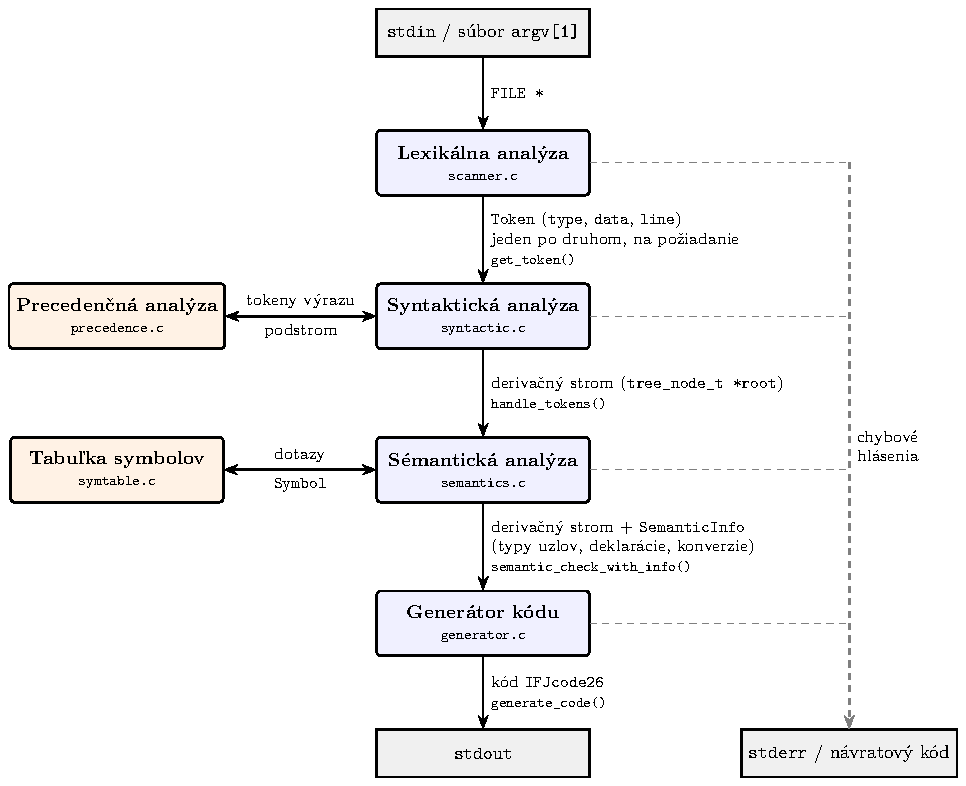
\includegraphics[width=0.9\linewidth]{architektura.pdf}
        \caption{Bloková architektúra prekladača (diagram vytvorený pomocou Claude Opus 5.5).}
        \label{fig:architektura}
\end{figure}

Syntaktický analyzátor si žiada tokeny od scannera na požiadanie a~stavia derivačný strom. Výrazy spracuje precedenčná analýza a vloží ich ako podstrom. Sémantická analýza ako jediná pracuje s~tabuľkou symbolov a~výsledky ukladá do \texttt{SemanticInfo}, z~ktorej spolu s~derivačným stromom generátor vytvorí kód \texttt{IFJcode26}.

\begin{table}[ht]
  \centering
  \setlength{\tabcolsep}{3pt}
  \renewcommand{\arraystretch}{1.2}
  \resizebox{\textwidth}{!}{%
  \begin{tabular}{|c||c|c|c|c|c|c|c|c|c|c|c|c|c|c|c|c|c|c|c|}
    \hline
    & $-_u$ & \texttt{!} & $*$ & $/$ & $+$ & $-$ & $<$ & $\leq$ & $>$ & $\geq$ & \texttt{==} & \texttt{!=} & \texttt{\&\&} & \texttt{||} & \texttt{.} & \texttt{(} & \texttt{)} & $i$ & \$ \\ \hline\hline
$-_u$ & $<$ & $<$ & $>$ & $>$ & $>$ & $>$ & $>$ & $>$ & $>$ & $>$ & $>$ & $>$ & $>$ & $>$ & $<$ & $<$ & $>$ & $<$ & $>$ \\ \hline
\texttt{!} & $<$ & $<$ & $>$ & $>$ & $>$ & $>$ & $>$ & $>$ & $>$ & $>$ & $>$ & $>$ & $>$ & $>$ & $<$ & $<$ & $>$ & $<$ & $>$ \\ \hline
$*$ & $<$ & $<$ & $>$ & $>$ & $>$ & $>$ & $>$ & $>$ & $>$ & $>$ & $>$ & $>$ & $>$ & $>$ & $<$ & $<$ & $>$ & $<$ & $>$ \\ \hline
$/$ & $<$ & $<$ & $>$ & $>$ & $>$ & $>$ & $>$ & $>$ & $>$ & $>$ & $>$ & $>$ & $>$ & $>$ & $<$ & $<$ & $>$ & $<$ & $>$ \\ \hline
$+$ & $<$ & $<$ & $<$ & $<$ & $>$ & $>$ & $>$ & $>$ & $>$ & $>$ & $>$ & $>$ & $>$ & $>$ & $<$ & $<$ & $>$ & $<$ & $>$ \\ \hline
$-$ & $<$ & $<$ & $<$ & $<$ & $>$ & $>$ & $>$ & $>$ & $>$ & $>$ & $>$ & $>$ & $>$ & $>$ & $<$ & $<$ & $>$ & $<$ & $>$ \\ \hline
$<$ & $<$ & $<$ & $<$ & $<$ & $<$ & $<$ &  &  &  &  & $>$ & $>$ & $>$ & $>$ & $<$ & $<$ & $>$ & $<$ & $>$ \\ \hline
$\leq$ & $<$ & $<$ & $<$ & $<$ & $<$ & $<$ &  &  &  &  & $>$ & $>$ & $>$ & $>$ & $<$ & $<$ & $>$ & $<$ & $>$ \\ \hline
$>$ & $<$ & $<$ & $<$ & $<$ & $<$ & $<$ &  &  &  &  & $>$ & $>$ & $>$ & $>$ & $<$ & $<$ & $>$ & $<$ & $>$ \\ \hline
$\geq$ & $<$ & $<$ & $<$ & $<$ & $<$ & $<$ &  &  &  &  & $>$ & $>$ & $>$ & $>$ & $<$ & $<$ & $>$ & $<$ & $>$ \\ \hline
\texttt{==} & $<$ & $<$ & $<$ & $<$ & $<$ & $<$ & $<$ & $<$ & $<$ & $<$ &  &  & $>$ & $>$ & $<$ & $<$ & $>$ & $<$ & $>$ \\ \hline
\texttt{!=} & $<$ & $<$ & $<$ & $<$ & $<$ & $<$ & $<$ & $<$ & $<$ & $<$ &  &  & $>$ & $>$ & $<$ & $<$ & $>$ & $<$ & $>$ \\ \hline
\texttt{\&\&} & $<$ & $<$ & $<$ & $<$ & $<$ & $<$ & $<$ & $<$ & $<$ & $<$ & $<$ & $<$ & $>$ & $>$ & $<$ & $<$ & $>$ & $<$ & $>$ \\ \hline
\texttt{||} & $<$ & $<$ & $<$ & $<$ & $<$ & $<$ & $<$ & $<$ & $<$ & $<$ & $<$ & $<$ & $<$ & $>$ & $<$ & $<$ & $>$ & $<$ & $>$ \\ \hline
\texttt{.} &  &  & $>$ & $>$ & $>$ & $>$ & $>$ & $>$ & $>$ & $>$ & $>$ & $>$ & $>$ & $>$ & $>$ &  & $>$ & $<$ & $>$ \\ \hline
\texttt{(} & $<$ & $<$ & $<$ & $<$ & $<$ & $<$ & $<$ & $<$ & $<$ & $<$ & $<$ & $<$ & $<$ & $<$ & $<$ & $<$ & $=$ & $<$ &  \\ \hline
\texttt{)} &  &  & $>$ & $>$ & $>$ & $>$ & $>$ & $>$ & $>$ & $>$ & $>$ & $>$ & $>$ & $>$ & $>$ &  & $>$ &  & $>$ \\ \hline
$i$ &  &  & $>$ & $>$ & $>$ & $>$ & $>$ & $>$ & $>$ & $>$ & $>$ & $>$ & $>$ & $>$ & $>$ &  & $>$ &  & $>$ \\ \hline
\$ & $<$ & $<$ & $<$ & $<$ & $<$ & $<$ & $<$ & $<$ & $<$ & $<$ & $<$ & $<$ & $<$ & $<$ & $<$ & $<$ &  & $<$ & \checkmark \\ \hline
\end{tabular}}
  \caption{Precedenčná tabuľka. Riadok je terminál na vrchole zásobníka, stĺpec je vstupný token.
    $<$~shift so zarážkou, $>$~redukcia, $=$~shift bez zarážky, prázdne políčko~syntaktická chyba,    \checkmark~prijatie výrazu. $-_u$ označuje unárne mínus, $i$~term
    (identifikátor, literál, \texttt{()}, \texttt{true}, \texttt{false}, volanie funkcie).}
  \label{tab:precedence}
\end{table}

\section{Lexikálna analýza}
Lexikálny analyzátor biele znaky na začiatku riadku preskočí. Po každom konci riadku porovná počet úvodných medzier s~uloženou históriou úrovní odsadenia a~podľa výsledku vygeneruje token \textsc{indent}, alebo za každú opustenú úroveň jeden token \textsc{dedent} (aj na konci súboru), vďaka čomu syntaktický analyzátor pracuje s~blokmi vymedzenými odsadením rovnako ako so zátvorkami. Lexikálna analýza je implementovaná podľa konečného automatu (obrázok \ref{fig:ka}).

\section{LL gramatika}
Syntaktický analyzátor (\texttt{syntactic.c}) je implementovaný rekurzívnym zostupom podľa nasledujúcej LL gramatiky. Pravidlá 58--61 (argumenty volania funkcie) sa spúšťajú z~precedenčnej syntaktickej analýzy, neterminály 62--66 rozkladá precedenčná syntaktická analýza (\texttt{precedence.c}) -- v~LL tabuľke nemajú vlastný riadok.

 
{\small
\setlength{\tabcolsep}{4pt}
\begin{longtable}{r l c >{\raggedright\arraybackslash}p{6.6cm} >{\raggedright\arraybackslash}p{3.2cm}}
1 & \textsf{PROGRAM} & $\rightarrow$ & \textsf{LEADING\_EOL} \textsf{PROLOG} \textsf{TOP\_LIST} \textsc{eof} & {\scriptsize } \\
2 & \textsf{PROLOG} & $\rightarrow$ & \texttt{import} \texttt{ifj26.*} \textsf{LINE\_END} & {\scriptsize } \\
3.1 & \textsf{TOP\_LIST} & $\rightarrow$ & \textsf{TOP\_ITEM} \textsf{TOP\_LIST} & {\scriptsize } \\
3.2 & \textsf{TOP\_LIST} & $\rightarrow$ & $\varepsilon$ & {\scriptsize } \\
4.1 & \textsf{TOP\_ITEM} & $\rightarrow$ & \texttt{@main} \textsf{ANNOTATION\_EOL} \textsf{FUNCTION\_DEF} & {\scriptsize } \\
4.2 & \textsf{TOP\_ITEM} & $\rightarrow$ & \textsf{FUNCTION\_DEF} & {\scriptsize } \\
4.3 & \textsf{TOP\_ITEM} & $\rightarrow$ & \textsf{TYPE\_DEF} & {\scriptsize } \\
4.4 & \textsf{TOP\_ITEM} & $\rightarrow$ & \textsf{CASE\_CLASS\_DEF} & {\scriptsize } \\
4.5 & \textsf{TOP\_ITEM} & $\rightarrow$ & \textsf{EXTENSION\_DEF} & {\scriptsize } \\
5.1 & \textsf{ANNOTATION\_EOL} & $\rightarrow$ & \textsc{eol} & {\scriptsize } \\
5.2 & \textsf{ANNOTATION\_EOL} & $\rightarrow$ & $\varepsilon$ & {\scriptsize } \\
6 & \textsf{FUNCTION\_DEF} & $\rightarrow$ & \texttt{def} \textit{identif} \textsf{PARAM\_LISTS} \textsf{OPTIONAL\_TYPE} \texttt{=} \textsf{RHS} \textsf{LINE\_END} & {\scriptsize } \\
7.1 & \textsf{PARAM\_LISTS} & $\rightarrow$ & \texttt{(} \textsf{PARAM\_LIST} \texttt{)} \textsf{PARAM\_LISTS} & {\scriptsize } \\
7.2 & \textsf{PARAM\_LISTS} & $\rightarrow$ & $\varepsilon$ & {\scriptsize } \\
8.1 & \textsf{PARAM\_LIST} & $\rightarrow$ & \textsf{PARAM} \textsf{PARAM\_LIST\_REST} & {\scriptsize } \\
8.2 & \textsf{PARAM\_LIST} & $\rightarrow$ & $\varepsilon$ & {\scriptsize } \\
9.1 & \textsf{PARAM\_LIST\_REST} & $\rightarrow$ & \texttt{,} \textsf{PARAM\_AFTER\_COMMA} & {\scriptsize } \\
9.2 & \textsf{PARAM\_LIST\_REST} & $\rightarrow$ & $\varepsilon$ & {\scriptsize } \\
10.1 & \textsf{PARAM\_AFTER\_COMMA} & $\rightarrow$ & \textsf{PARAM} \textsf{PARAM\_LIST\_REST} & {\scriptsize } \\
10.2 & \textsf{PARAM\_AFTER\_COMMA} & $\rightarrow$ & $\varepsilon$ & {\scriptsize \textit{koncová čiarka, len ak je medzi ',' a ')' koniec riadku (lookahead ')' a newline\_before)}} \\
11 & \textsf{PARAM} & $\rightarrow$ & \textit{identif} \texttt{:} \textsf{TYPE} & {\scriptsize } \\
12.1 & \textsf{OPTIONAL\_TYPE} & $\rightarrow$ & \texttt{:} \textsf{TYPE} & {\scriptsize } \\
12.2 & \textsf{OPTIONAL\_TYPE} & $\rightarrow$ & $\varepsilon$ & {\scriptsize } \\
13 & \textsf{TYPE} & $\rightarrow$ & \textsf{SIMPLE\_TYPE} \textsf{UNION\_REST} & {\scriptsize } \\
14.1 & \textsf{UNION\_REST} & $\rightarrow$ & \texttt{|} \textsf{SIMPLE\_TYPE} \textsf{UNION\_REST} & {\scriptsize } \\
14.2 & \textsf{UNION\_REST} & $\rightarrow$ & $\varepsilon$ & {\scriptsize } \\
15.1 & \textsf{SIMPLE\_TYPE} & $\rightarrow$ & \texttt{Int} & {\scriptsize } \\
15.2 & \textsf{SIMPLE\_TYPE} & $\rightarrow$ & \texttt{Double} & {\scriptsize } \\
15.3 & \textsf{SIMPLE\_TYPE} & $\rightarrow$ & \texttt{String} & {\scriptsize } \\
15.4 & \textsf{SIMPLE\_TYPE} & $\rightarrow$ & \texttt{Unit} & {\scriptsize } \\
15.5 & \textsf{SIMPLE\_TYPE} & $\rightarrow$ & \texttt{Boolean} & {\scriptsize } \\
15.6 & \textsf{SIMPLE\_TYPE} & $\rightarrow$ & \textit{identif} & {\scriptsize } \\
16 & \textsf{TYPE\_DEF} & $\rightarrow$ & \texttt{type} \textit{identif} \texttt{=} \textsf{TYPE} \textsf{LINE\_END} & {\scriptsize } \\
17 & \textsf{CASE\_CLASS\_DEF} & $\rightarrow$ & \texttt{case} \texttt{class} \textit{identif} \texttt{(} \textsf{PARAM\_LIST} \texttt{)} \textsf{LINE\_END} & {\scriptsize } \\
18 & \textsf{EXTENSION\_DEF} & $\rightarrow$ & \texttt{extension} \texttt{(} \textsf{PARAM} \texttt{)} \textsc{eol} \textsc{indent} \textsf{METHOD\_LIST} \textsf{BLOCK\_END} \textsf{LINE\_END} & {\scriptsize } \\
19 & \textsf{METHOD\_LIST} & $\rightarrow$ & \textsf{FUNCTION\_DEF} \textsf{METHOD\_LIST\_REST} & {\scriptsize } \\
20.1 & \textsf{METHOD\_LIST\_REST} & $\rightarrow$ & \textsf{FUNCTION\_DEF} \textsf{METHOD\_LIST\_REST} & {\scriptsize } \\
20.2 & \textsf{METHOD\_LIST\_REST} & $\rightarrow$ & $\varepsilon$ & {\scriptsize } \\
21.1 & \textsf{RHS} & $\rightarrow$ & \textsf{BLOCK} & {\scriptsize } \\
21.2 & \textsf{RHS} & $\rightarrow$ & \textsf{VALUE} & {\scriptsize } \\
22 & \textsf{BLOCK} & $\rightarrow$ & \textsc{eol} \textsc{indent} \textsf{STATEMENT\_LIST} \textsf{BLOCK\_END} & {\scriptsize } \\
23 & \textsf{STATEMENT\_LIST} & $\rightarrow$ & \textsf{STATEMENT\_LINE} \textsf{STATEMENT\_LIST\_REST} & {\scriptsize } \\
24.1 & \textsf{STATEMENT\_LIST\_REST} & $\rightarrow$ & \textsf{STATEMENT\_LINE} \textsf{STATEMENT\_LIST\_REST} & {\scriptsize } \\
24.2 & \textsf{STATEMENT\_LIST\_REST} & $\rightarrow$ & $\varepsilon$ & {\scriptsize } \\
25 & \textsf{STATEMENT\_LINE} & $\rightarrow$ & \textsf{STATEMENT} \textsf{STATEMENT\_LINE\_REST} & {\scriptsize } \\
26.1 & \textsf{STATEMENT\_LINE\_REST} & $\rightarrow$ & \texttt{;} \textsf{STATEMENT} \textsf{STATEMENT\_LINE\_REST} & {\scriptsize } \\
26.2 & \textsf{STATEMENT\_LINE\_REST} & $\rightarrow$ & \textsf{LINE\_END} & {\scriptsize } \\
27.1 & \textsf{STATEMENT} & $\rightarrow$ & \textsf{VAR\_DEFINITION} & {\scriptsize } \\
27.2 & \textsf{STATEMENT} & $\rightarrow$ & \textsf{INLINE\_STATEMENT} & {\scriptsize } \\
28.1 & \textsf{INLINE\_STATEMENT} & $\rightarrow$ & \textsf{RETURN\_STATEMENT} & {\scriptsize } \\
28.2 & \textsf{INLINE\_STATEMENT} & $\rightarrow$ & \textsf{IF\_STATEMENT} & {\scriptsize } \\
28.3 & \textsf{INLINE\_STATEMENT} & $\rightarrow$ & \textsf{WHILE\_STATEMENT} & {\scriptsize } \\
28.4 & \textsf{INLINE\_STATEMENT} & $\rightarrow$ & \textsf{FOR\_STATEMENT} & {\scriptsize } \\
28.5 & \textsf{INLINE\_STATEMENT} & $\rightarrow$ & \textit{identif} \textsf{ID\_STATEMENT} & {\scriptsize } \\
28.6 & \textsf{INLINE\_STATEMENT} & $\rightarrow$ & \textsf{EXPRESSION\_NOID} \textsf{MATCH\_SUFFIX} & {\scriptsize } \\
29 & \textsf{VAR\_DEFINITION} & $\rightarrow$ & \textsf{VAR\_KIND} \textit{identif} \textsf{OPTIONAL\_TYPE} \texttt{=} \textsf{RHS} & {\scriptsize } \\
30.1 & \textsf{VAR\_KIND} & $\rightarrow$ & \texttt{val} & {\scriptsize } \\
30.2 & \textsf{VAR\_KIND} & $\rightarrow$ & \texttt{var} & {\scriptsize } \\
31.1 & \textsf{ID\_STATEMENT} & $\rightarrow$ & \texttt{=} \textsf{RHS} & {\scriptsize } \\
31.2 & \textsf{ID\_STATEMENT} & $\rightarrow$ & \textsf{EXPRESSION\_AFTER\_ID} \textsf{MATCH\_SUFFIX} & {\scriptsize } \\
32 & \textsf{RETURN\_STATEMENT} & $\rightarrow$ & \texttt{return} \textsf{RETURN\_VALUE} & {\scriptsize } \\
33.1 & \textsf{RETURN\_VALUE} & $\rightarrow$ & \textsf{VALUE} & {\scriptsize } \\
33.2 & \textsf{RETURN\_VALUE} & $\rightarrow$ & $\varepsilon$ & {\scriptsize } \\
34 & \textsf{IF\_STATEMENT} & $\rightarrow$ & \texttt{if} \textsf{EXPRESSION} \texttt{then} \textsf{BODY} \textsf{ELSE\_PART} & {\scriptsize } \\
35.1 & \textsf{ELSE\_PART} & $\rightarrow$ & \texttt{else} \textsf{BODY} & {\scriptsize } \\
35.2 & \textsf{ELSE\_PART} & $\rightarrow$ & $\varepsilon$ & {\scriptsize } \\
36 & \textsf{WHILE\_STATEMENT} & $\rightarrow$ & \texttt{while} \textsf{EXPRESSION} \texttt{do} \textsf{BODY} & {\scriptsize } \\
37.1 & \textsf{BODY} & $\rightarrow$ & \textsf{BLOCK} & {\scriptsize } \\
37.2 & \textsf{BODY} & $\rightarrow$ & \textsf{INLINE\_STATEMENT} & {\scriptsize } \\
37.3 & \textsf{BODY} & $\rightarrow$ & \textsf{EXPRESSION\_UNARY} & {\scriptsize } \\
38 & \textsf{FOR\_STATEMENT} & $\rightarrow$ & \texttt{for} \textsf{FOR\_HEADER} \texttt{do} \textsf{BODY} & {\scriptsize } \\
39.1 & \textsf{FOR\_HEADER} & $\rightarrow$ & \textsf{GENERATOR} \textsf{INLINE\_GUARDS} & {\scriptsize } \\
39.2 & \textsf{FOR\_HEADER} & $\rightarrow$ & \textsc{eol} \textsc{indent} \textsf{GENERATOR} \textsf{INLINE\_GUARDS} \textsc{eol} \textsf{GUARD\_LINES} \textsc{dedent} & {\scriptsize } \\
40 & \textsf{GENERATOR} & $\rightarrow$ & \textit{identif} \texttt{<-} \textsf{EXPRESSION} \textsf{RANGE\_OP} \textsf{EXPRESSION} \textsf{STEP} & {\scriptsize } \\
41.1 & \textsf{RANGE\_OP} & $\rightarrow$ & \texttt{to} & {\scriptsize } \\
41.2 & \textsf{RANGE\_OP} & $\rightarrow$ & \texttt{until} & {\scriptsize } \\
42.1 & \textsf{STEP} & $\rightarrow$ & \texttt{by} \textsf{EXPRESSION} & {\scriptsize } \\
42.2 & \textsf{STEP} & $\rightarrow$ & $\varepsilon$ & {\scriptsize } \\
43.1 & \textsf{INLINE\_GUARDS} & $\rightarrow$ & \texttt{if} \textsf{EXPRESSION} \textsf{INLINE\_GUARDS} & {\scriptsize } \\
43.2 & \textsf{INLINE\_GUARDS} & $\rightarrow$ & $\varepsilon$ & {\scriptsize } \\
44.1 & \textsf{GUARD\_LINES} & $\rightarrow$ & \texttt{if} \textsf{EXPRESSION} \textsf{INLINE\_GUARDS} \textsc{eol} \textsf{GUARD\_LINES} & {\scriptsize } \\
44.2 & \textsf{GUARD\_LINES} & $\rightarrow$ & $\varepsilon$ & {\scriptsize } \\
45.1 & \textsf{VALUE} & $\rightarrow$ & \textsf{IF\_STATEMENT} & {\scriptsize } \\
45.2 & \textsf{VALUE} & $\rightarrow$ & \textsf{VALUE\_EXPRESSION} \textsf{MATCH\_SUFFIX} & {\scriptsize } \\
46.1 & \textsf{MATCH\_SUFFIX} & $\rightarrow$ & \texttt{match} \textsc{eol} \textsc{indent} \textsf{CASE\_LIST} \textsf{BLOCK\_END} & {\scriptsize } \\
46.2 & \textsf{MATCH\_SUFFIX} & $\rightarrow$ & $\varepsilon$ & {\scriptsize } \\
47 & \textsf{CASE\_LIST} & $\rightarrow$ & \textsf{CASE\_CLAUSE} \textsf{CASE\_LIST\_REST} & {\scriptsize } \\
48.1 & \textsf{CASE\_LIST\_REST} & $\rightarrow$ & \textsf{CASE\_CLAUSE} \textsf{CASE\_LIST\_REST} & {\scriptsize } \\
48.2 & \textsf{CASE\_LIST\_REST} & $\rightarrow$ & $\varepsilon$ & {\scriptsize } \\
49 & \textsf{CASE\_CLAUSE} & $\rightarrow$ & \texttt{case} \textsf{PATTERN} \textsf{CASE\_GUARD} \texttt{=>} \textsf{RHS} \textsf{LINE\_END} & {\scriptsize } \\
50.1 & \textsf{CASE\_GUARD} & $\rightarrow$ & \texttt{if} \textsf{EXPRESSION} & {\scriptsize } \\
50.2 & \textsf{CASE\_GUARD} & $\rightarrow$ & $\varepsilon$ & {\scriptsize } \\
51.1 & \textsf{PATTERN} & $\rightarrow$ & \texttt{\_} & {\scriptsize } \\
51.2 & \textsf{PATTERN} & $\rightarrow$ & \textit{identif} \textsf{ID\_PATTERN} & {\scriptsize } \\
51.3 & \textsf{PATTERN} & $\rightarrow$ & \textsf{LITERAL\_PATTERN} & {\scriptsize } \\
52.1 & \textsf{ID\_PATTERN} & $\rightarrow$ & \texttt{:} \textsf{TYPE} & {\scriptsize } \\
52.2 & \textsf{ID\_PATTERN} & $\rightarrow$ & \texttt{(} \textsf{SUBPATTERN\_LIST} \texttt{)} & {\scriptsize } \\
53.1 & \textsf{SUBPATTERN\_LIST} & $\rightarrow$ & \textsf{SUBPATTERN} \textsf{SUBPATTERN\_REST} & {\scriptsize } \\
53.2 & \textsf{SUBPATTERN\_LIST} & $\rightarrow$ & $\varepsilon$ & {\scriptsize } \\
54.1 & \textsf{SUBPATTERN\_REST} & $\rightarrow$ & \texttt{,} \textsf{SUBPATTERN} \textsf{SUBPATTERN\_REST} & {\scriptsize } \\
54.2 & \textsf{SUBPATTERN\_REST} & $\rightarrow$ & $\varepsilon$ & {\scriptsize } \\
55.1 & \textsf{SUBPATTERN} & $\rightarrow$ & \textit{identif} & {\scriptsize } \\
55.2 & \textsf{SUBPATTERN} & $\rightarrow$ & \texttt{\_} & {\scriptsize } \\
55.3 & \textsf{SUBPATTERN} & $\rightarrow$ & \textsf{LITERAL\_PATTERN} & {\scriptsize } \\
56.1 & \textsf{LITERAL\_PATTERN} & $\rightarrow$ & \textit{int\_lit} & {\scriptsize } \\
56.2 & \textsf{LITERAL\_PATTERN} & $\rightarrow$ & \textit{double\_lit} & {\scriptsize } \\
56.3 & \textsf{LITERAL\_PATTERN} & $\rightarrow$ & \textit{string\_lit} & {\scriptsize } \\
56.4 & \textsf{LITERAL\_PATTERN} & $\rightarrow$ & \textit{bool\_lit} & {\scriptsize } \\
56.5 & \textsf{LITERAL\_PATTERN} & $\rightarrow$ & \texttt{-} \textsf{NUMBER} & {\scriptsize } \\
56.6 & \textsf{LITERAL\_PATTERN} & $\rightarrow$ & \texttt{(} \texttt{)} & {\scriptsize } \\
57.1 & \textsf{NUMBER} & $\rightarrow$ & \textit{int\_lit} & {\scriptsize } \\
57.2 & \textsf{NUMBER} & $\rightarrow$ & \textit{double\_lit} & {\scriptsize } \\
58 & \textsf{CALL\_ARGS} & $\rightarrow$ & \texttt{(} \textsf{ARG\_LIST} \texttt{)} & {\scriptsize } \\
59.1 & \textsf{ARG\_LIST} & $\rightarrow$ & \textsf{VALUE} \textsf{ARG\_LIST\_REST} & {\scriptsize } \\
59.2 & \textsf{ARG\_LIST} & $\rightarrow$ & $\varepsilon$ & {\scriptsize } \\
60.1 & \textsf{ARG\_LIST\_REST} & $\rightarrow$ & \texttt{,} \textsf{ARG\_AFTER\_COMMA} & {\scriptsize } \\
60.2 & \textsf{ARG\_LIST\_REST} & $\rightarrow$ & $\varepsilon$ & {\scriptsize } \\
61.1 & \textsf{ARG\_AFTER\_COMMA} & $\rightarrow$ & \textsf{VALUE} \textsf{ARG\_LIST\_REST} & {\scriptsize } \\
61.2 & \textsf{ARG\_AFTER\_COMMA} & $\rightarrow$ & $\varepsilon$ & {\scriptsize \textit{koncová čiarka}} \\
62 & \textsf{EXPRESSION} & $\rightarrow$ & \textit{precedenčná syntaktická analýza} & \\
63 & \textsf{VALUE\_EXPRESSION} & $\rightarrow$ & \textit{precedenčná syntaktická analýza} & \\
64 & \textsf{EXPRESSION\_AFTER\_ID} & $\rightarrow$ & \textit{precedenčná syntaktická analýza} & \\
65 & \textsf{EXPRESSION\_NOID} & $\rightarrow$ & \textit{precedenčná syntaktická analýza} & \\
66 & \textsf{EXPRESSION\_UNARY} & $\rightarrow$ & \textit{precedenčná syntaktická analýza} & \\
67.1 & \textsf{LEADING\_EOL} & $\rightarrow$ & \textsc{eol} \textsf{LEADING\_EOL} & {\scriptsize } \\
67.2 & \textsf{LEADING\_EOL} & $\rightarrow$ & $\varepsilon$ & {\scriptsize } \\
68 & \textsf{BLOCK\_END} & $\rightarrow$ & \textsc{dedent} & {\scriptsize \textit{lexer na konci súboru posiela DEDENT pre každý otvorený blok}} \\
69.1 & \textsf{LINE\_END} & $\rightarrow$ & \textsc{eol} & {\scriptsize } \\
69.2 & \textsf{LINE\_END} & $\rightarrow$ & $\varepsilon$ & {\scriptsize \textit{lookahead EOF alebo DEDENT (posledný riadok bez LF), alebo predchádzajúci token bol DEDENT (riadok ukončil blok), nič sa nespotrebuje}} \\
\end{longtable}
}
 
\section{LL tabuľka}
LL tabuľka je kvôli veľkosti rozdelená na štyri časti (tabuľky~\ref{tab:ll1}--\ref{tab:ll4}): prvé dve obsahujú prvú polovicu terminálov, posledné dve druhú. Neterminály a~terminály, ktoré v~danej časti nemajú žiadne pravidlo, v~nej nie sú uvedené. 
 
\begin{itemize}
  \item \textit{op} -- binárny operátor okrem \texttt{-}: \texttt{+ * / < <= > >= == != \&\& ||}.
  \item Terminály \textsc{indent}, \texttt{ifj26.*}, \texttt{class}, \texttt{then} a~\texttt{<-} sa nikdy nepoužívajú na výber pravidla (vyskytujú sa len na pevnom mieste v~pravidle), ich stĺpce v~tabuľke nie sú.
  \item $^{a}$ -- pravidlo 69.2 sa pri tomto tokene použije, len ak predchádzajúci token bol \textsc{dedent} (riadok ukončil blok). Pri \textsc{eof} a~\textsc{dedent} sa použije vždy.
  \item \textsf{RETURN\_VALUE}: prázdna návratová hodnota (33.2) sa použije pre \textsc{eol}, \texttt{;}, \texttt{else}, \texttt{,}, \texttt{)}, \textsc{dedent} a~\textsc{eof}, pre začiatok hodnoty vždy 33.1.
\end{itemize}
 
\begin{sidewaystable}
\centering
\scriptsize
\setlength{\tabcolsep}{3.10pt}
\renewcommand{\arraystretch}{1.151}
\begin{adjustbox}{width=\textheight, totalheight=15.5cm, keepaspectratio}
\begin{tabular}{|l|>{\centering\arraybackslash}p{19pt}|>{\centering\arraybackslash}p{19pt}|>{\centering\arraybackslash}p{19pt}|>{\centering\arraybackslash}p{19pt}|>{\centering\arraybackslash}p{19pt}|>{\centering\arraybackslash}p{19pt}|>{\centering\arraybackslash}p{19pt}|>{\centering\arraybackslash}p{19pt}|>{\centering\arraybackslash}p{19pt}|>{\centering\arraybackslash}p{19pt}|>{\centering\arraybackslash}p{19pt}|>{\centering\arraybackslash}p{19pt}|>{\centering\arraybackslash}p{19pt}|>{\centering\arraybackslash}p{19pt}|>{\centering\arraybackslash}p{19pt}|>{\centering\arraybackslash}p{19pt}|>{\centering\arraybackslash}p{19pt}|>{\centering\arraybackslash}p{19pt}|>{\centering\arraybackslash}p{19pt}|}
\hline
 & \rotatebox{90}{\textsc{eol}} & \rotatebox{90}{\textsc{dedent}} & \rotatebox{90}{\textsc{eof}} & \rotatebox{90}{\texttt{import}} & \rotatebox{90}{\texttt{@main}} & \rotatebox{90}{\texttt{def}} & \rotatebox{90}{\texttt{type}} & \rotatebox{90}{\texttt{case}} & \rotatebox{90}{\texttt{extension}} & \rotatebox{90}{\texttt{val}} & \rotatebox{90}{\texttt{var}} & \rotatebox{90}{\texttt{return}} & \rotatebox{90}{\texttt{if}} & \rotatebox{90}{\texttt{else}} & \rotatebox{90}{\texttt{while}} & \rotatebox{90}{\texttt{for}} & \rotatebox{90}{\texttt{match}} & \rotatebox{90}{\textit{identif}} & \rotatebox{90}{\textit{int\_lit}} \\ \hline\hline
\textsf{PROGRAM} & 1 &  &  & 1 &  &  &  &  &  &  &  &  &  &  &  &  &  &  &  \\ \hline
\textsf{PROLOG} &  &  &  & 2 &  &  &  &  &  &  &  &  &  &  &  &  &  &  &  \\ \hline
\textsf{TOP\_LIST} &  &  & 3.2 &  & 3.1 & 3.1 & 3.1 & 3.1 & 3.1 &  &  &  &  &  &  &  &  &  &  \\ \hline
\textsf{TOP\_ITEM} &  &  &  &  & 4.1 & 4.2 & 4.3 & 4.4 & 4.5 &  &  &  &  &  &  &  &  &  &  \\ \hline
\textsf{ANNOTATION\_EOL} & 5.1 &  &  &  &  & 5.2 &  &  &  &  &  &  &  &  &  &  &  &  &  \\ \hline
\textsf{FUNCTION\_DEF} &  &  &  &  &  & 6 &  &  &  &  &  &  &  &  &  &  &  &  &  \\ \hline
\textsf{PARAM\_LIST} &  &  &  &  &  &  &  &  &  &  &  &  &  &  &  &  &  & 8.1 &  \\ \hline
\textsf{PARAM\_AFTER\_COMMA} &  &  &  &  &  &  &  &  &  &  &  &  &  &  &  &  &  & 10.1 &  \\ \hline
\textsf{PARAM} &  &  &  &  &  &  &  &  &  &  &  &  &  &  &  &  &  & 11 &  \\ \hline
\textsf{TYPE} &  &  &  &  &  &  &  &  &  &  &  &  &  &  &  &  &  & 13 &  \\ \hline
\textsf{UNION\_REST} & 14.2 &  & 14.2 &  & 14.2 & 14.2 & 14.2 & 14.2 & 14.2 &  &  &  & 14.2 &  &  &  &  &  &  \\ \hline
\textsf{SIMPLE\_TYPE} &  &  &  &  &  &  &  &  &  &  &  &  &  &  &  &  &  & 15.6 &  \\ \hline
\textsf{TYPE\_DEF} &  &  &  &  &  &  & 16 &  &  &  &  &  &  &  &  &  &  &  &  \\ \hline
\textsf{CASE\_CLASS\_DEF} &  &  &  &  &  &  &  & 17 &  &  &  &  &  &  &  &  &  &  &  \\ \hline
\textsf{EXTENSION\_DEF} &  &  &  &  &  &  &  &  & 18 &  &  &  &  &  &  &  &  &  &  \\ \hline
\textsf{METHOD\_LIST} &  &  &  &  &  & 19 &  &  &  &  &  &  &  &  &  &  &  &  &  \\ \hline
\textsf{METHOD\_LIST\_REST} &  & 20.2 &  &  &  & 20.1 &  &  &  &  &  &  &  &  &  &  &  &  &  \\ \hline
\textsf{RHS} & 21.1 &  &  &  &  &  &  &  &  &  &  &  & 21.2 &  &  &  &  & 21.2 & 21.2 \\ \hline
\textsf{BLOCK} & 22 &  &  &  &  &  &  &  &  &  &  &  &  &  &  &  &  &  &  \\ \hline
\textsf{STATEMENT\_LIST} &  &  &  &  &  &  &  &  &  & 23 & 23 & 23 & 23 &  & 23 & 23 &  & 23 & 23 \\ \hline
\textsf{STATEMENT\_LIST\_REST} &  & 24.2 &  &  &  &  &  &  &  & 24.1 & 24.1 & 24.1 & 24.1 &  & 24.1 & 24.1 &  & 24.1 & 24.1 \\ \hline
\textsf{STATEMENT\_LINE} &  &  &  &  &  &  &  &  &  & 25 & 25 & 25 & 25 &  & 25 & 25 &  & 25 & 25 \\ \hline
\textsf{STATEMENT\_LINE\_REST} & 26.2 & 26.2 &  &  &  &  &  &  &  & 26.2 & 26.2 & 26.2 & 26.2 &  & 26.2 & 26.2 &  & 26.2 & 26.2 \\ \hline
\textsf{STATEMENT} &  &  &  &  &  &  &  &  &  & 27.1 & 27.1 & 27.2 & 27.2 &  & 27.2 & 27.2 &  & 27.2 & 27.2 \\ \hline
\textsf{INLINE\_STATEMENT} &  &  &  &  &  &  &  &  &  &  &  & 28.1 & 28.2 &  & 28.3 & 28.4 &  & 28.5 & 28.6 \\ \hline
\textsf{VAR\_DEFINITION} &  &  &  &  &  &  &  &  &  & 29 & 29 &  &  &  &  &  &  &  &  \\ \hline
\textsf{VAR\_KIND} &  &  &  &  &  &  &  &  &  & 30.1 & 30.2 &  &  &  &  &  &  &  &  \\ \hline
\textsf{ID\_STATEMENT} & 31.2 & 31.2 & 31.2 &  & 31.2 & 31.2 & 31.2 & 31.2 & 31.2 & 31.2 & 31.2 & 31.2 & 31.2 & 31.2 & 31.2 & 31.2 & 31.2 & 31.2 & 31.2 \\ \hline
\textsf{RETURN\_STATEMENT} &  &  &  &  &  &  &  &  &  &  &  & 32 &  &  &  &  &  &  &  \\ \hline
\end{tabular}
\end{adjustbox}
\caption{LL tabuľka, 1.~časť zo~4 -- terminály \textsc{eol} až \textit{int\_lit}, neterminály \textsf{PROGRAM} až \textsf{RETURN\_STATEMENT}}
\label{tab:ll1}
\end{sidewaystable}
 
\begin{sidewaystable}
\centering
\scriptsize
\setlength{\tabcolsep}{2.50pt}
\renewcommand{\arraystretch}{1.335}
\begin{adjustbox}{width=\textheight, totalheight=15.5cm, keepaspectratio}
\begin{tabular}{|l|>{\centering\arraybackslash}p{19pt}|>{\centering\arraybackslash}p{19pt}|>{\centering\arraybackslash}p{19pt}|>{\centering\arraybackslash}p{19pt}|>{\centering\arraybackslash}p{19pt}|>{\centering\arraybackslash}p{19pt}|>{\centering\arraybackslash}p{19pt}|>{\centering\arraybackslash}p{19pt}|>{\centering\arraybackslash}p{19pt}|>{\centering\arraybackslash}p{19pt}|>{\centering\arraybackslash}p{19pt}|>{\centering\arraybackslash}p{19pt}|>{\centering\arraybackslash}p{19pt}|>{\centering\arraybackslash}p{19pt}|>{\centering\arraybackslash}p{19pt}|>{\centering\arraybackslash}p{19pt}|>{\centering\arraybackslash}p{19pt}|>{\centering\arraybackslash}p{19pt}|>{\centering\arraybackslash}p{19pt}|>{\centering\arraybackslash}p{19pt}|>{\centering\arraybackslash}p{19pt}|>{\centering\arraybackslash}p{19pt}|>{\centering\arraybackslash}p{19pt}|}
\hline
 & \rotatebox{90}{\textsc{eol}} & \rotatebox{90}{\textsc{dedent}} & \rotatebox{90}{\textsc{eof}} & \rotatebox{90}{\texttt{import}} & \rotatebox{90}{\texttt{@main}} & \rotatebox{90}{\texttt{def}} & \rotatebox{90}{\texttt{type}} & \rotatebox{90}{\texttt{case}} & \rotatebox{90}{\texttt{extension}} & \rotatebox{90}{\texttt{val}} & \rotatebox{90}{\texttt{var}} & \rotatebox{90}{\texttt{return}} & \rotatebox{90}{\texttt{if}} & \rotatebox{90}{\texttt{else}} & \rotatebox{90}{\texttt{while}} & \rotatebox{90}{\texttt{do}} & \rotatebox{90}{\texttt{for}} & \rotatebox{90}{\texttt{to}} & \rotatebox{90}{\texttt{until}} & \rotatebox{90}{\texttt{by}} & \rotatebox{90}{\texttt{match}} & \rotatebox{90}{\textit{identif}} & \rotatebox{90}{\textit{int\_lit}} \\ \hline\hline
\textsf{RETURN\_VALUE} & 33.2 & 33.2 & 33.2 &  &  &  &  &  &  &  &  &  & 33.1 & 33.2 &  &  &  &  &  &  &  & 33.1 & 33.1 \\ \hline
\textsf{IF\_STATEMENT} &  &  &  &  &  &  &  &  &  &  &  &  & 34 &  &  &  &  &  &  &  &  &  &  \\ \hline
\textsf{ELSE\_PART} & 35.2 & 35.2 & 35.2 &  & 35.2 & 35.2 & 35.2 & 35.2 & 35.2 & 35.2 & 35.2 & 35.2 & 35.2 & 35.1 & 35.2 &  & 35.2 &  &  &  &  & 35.2 & 35.2 \\ \hline
\textsf{WHILE\_STATEMENT} &  &  &  &  &  &  &  &  &  &  &  &  &  &  & 36 &  &  &  &  &  &  &  &  \\ \hline
\textsf{BODY} & 37.1 &  &  &  &  &  &  &  &  &  &  & 37.2 & 37.2 &  & 37.2 &  & 37.2 &  &  &  &  & 37.2 & 37.2 \\ \hline
\textsf{FOR\_STATEMENT} &  &  &  &  &  &  &  &  &  &  &  &  &  &  &  &  & 38 &  &  &  &  &  &  \\ \hline
\textsf{FOR\_HEADER} & 39.2 &  &  &  &  &  &  &  &  &  &  &  &  &  &  &  &  &  &  &  &  & 39.1 &  \\ \hline
\textsf{GENERATOR} &  &  &  &  &  &  &  &  &  &  &  &  &  &  &  &  &  &  &  &  &  & 40 &  \\ \hline
\textsf{RANGE\_OP} &  &  &  &  &  &  &  &  &  &  &  &  &  &  &  &  &  & 41.1 & 41.2 &  &  &  &  \\ \hline
\textsf{STEP} & 42.2 &  &  &  &  &  &  &  &  &  &  &  & 42.2 &  &  & 42.2 &  &  &  & 42.1 &  &  &  \\ \hline
\textsf{INLINE\_GUARDS} & 43.2 &  &  &  &  &  &  &  &  &  &  &  & 43.1 &  &  & 43.2 &  &  &  &  &  &  &  \\ \hline
\textsf{GUARD\_LINES} &  & 44.2 &  &  &  &  &  &  &  &  &  &  & 44.1 &  &  &  &  &  &  &  &  &  &  \\ \hline
\textsf{VALUE} &  &  &  &  &  &  &  &  &  &  &  &  & 45.1 &  &  &  &  &  &  &  &  & 45.2 & 45.2 \\ \hline
\textsf{MATCH\_SUFFIX} & 46.2 & 46.2 & 46.2 &  & 46.2 & 46.2 & 46.2 & 46.2 & 46.2 & 46.2 & 46.2 & 46.2 & 46.2 & 46.2 & 46.2 &  & 46.2 &  &  &  & 46.1 & 46.2 & 46.2 \\ \hline
\textsf{CASE\_LIST} &  &  &  &  &  &  &  & 47 &  &  &  &  &  &  &  &  &  &  &  &  &  &  &  \\ \hline
\textsf{CASE\_LIST\_REST} &  & 48.2 &  &  &  &  &  & 48.1 &  &  &  &  &  &  &  &  &  &  &  &  &  &  &  \\ \hline
\textsf{CASE\_CLAUSE} &  &  &  &  &  &  &  & 49 &  &  &  &  &  &  &  &  &  &  &  &  &  &  &  \\ \hline
\textsf{CASE\_GUARD} &  &  &  &  &  &  &  &  &  &  &  &  & 50.1 &  &  &  &  &  &  &  &  &  &  \\ \hline
\textsf{PATTERN} &  &  &  &  &  &  &  &  &  &  &  &  &  &  &  &  &  &  &  &  &  & 51.2 & 51.3 \\ \hline
\textsf{SUBPATTERN\_LIST} &  &  &  &  &  &  &  &  &  &  &  &  &  &  &  &  &  &  &  &  &  & 53.1 & 53.1 \\ \hline
\textsf{SUBPATTERN} &  &  &  &  &  &  &  &  &  &  &  &  &  &  &  &  &  &  &  &  &  & 55.1 & 55.3 \\ \hline
\textsf{LITERAL\_PATTERN} &  &  &  &  &  &  &  &  &  &  &  &  &  &  &  &  &  &  &  &  &  &  & 56.1 \\ \hline
\textsf{NUMBER} &  &  &  &  &  &  &  &  &  &  &  &  &  &  &  &  &  &  &  &  &  &  & 57.1 \\ \hline
\textsf{ARG\_LIST} &  &  &  &  &  &  &  &  &  &  &  &  & 59.1 &  &  &  &  &  &  &  &  & 59.1 & 59.1 \\ \hline
\textsf{ARG\_AFTER\_COMMA} &  &  &  &  &  &  &  &  &  &  &  &  & 61.1 &  &  &  &  &  &  &  &  & 61.1 & 61.1 \\ \hline
\textsf{LEADING\_EOL} & 67.1 &  &  & 67.2 &  &  &  &  &  &  &  &  &  &  &  &  &  &  &  &  &  &  &  \\ \hline
\textsf{BLOCK\_END} &  & 68 &  &  &  &  &  &  &  &  &  &  &  &  &  &  &  &  &  &  &  &  &  \\ \hline
\textsf{LINE\_END} & 69.1 & 69.2 & 69.2 &  & 69.2$^{a}$ & 69.2$^{a}$ & 69.2$^{a}$ & 69.2$^{a}$ & 69.2$^{a}$ & 69.2$^{a}$ & 69.2$^{a}$ & 69.2$^{a}$ & 69.2$^{a}$ &  & 69.2$^{a}$ &  & 69.2$^{a}$ &  &  &  &  & 69.2$^{a}$ & 69.2$^{a}$ \\ \hline
\end{tabular}
\end{adjustbox}
\caption{LL tabuľka, 2.~časť zo~4 -- terminály \textsc{eol} až \textit{int\_lit}, neterminály \textsf{RETURN\_VALUE} až \textsf{LINE\_END}}
\label{tab:ll2}
\end{sidewaystable}
 
\begin{sidewaystable}
\centering
\scriptsize
\setlength{\tabcolsep}{2.51pt}
\renewcommand{\arraystretch}{2.206}
\begin{adjustbox}{width=\textheight, totalheight=15.5cm, keepaspectratio}
\begin{tabular}{|l|>{\centering\arraybackslash}p{19pt}|>{\centering\arraybackslash}p{19pt}|>{\centering\arraybackslash}p{19pt}|>{\centering\arraybackslash}p{19pt}|>{\centering\arraybackslash}p{19pt}|>{\centering\arraybackslash}p{19pt}|>{\centering\arraybackslash}p{19pt}|>{\centering\arraybackslash}p{19pt}|>{\centering\arraybackslash}p{19pt}|>{\centering\arraybackslash}p{19pt}|>{\centering\arraybackslash}p{19pt}|>{\centering\arraybackslash}p{19pt}|>{\centering\arraybackslash}p{19pt}|>{\centering\arraybackslash}p{19pt}|>{\centering\arraybackslash}p{19pt}|>{\centering\arraybackslash}p{19pt}|>{\centering\arraybackslash}p{19pt}|>{\centering\arraybackslash}p{19pt}|>{\centering\arraybackslash}p{19pt}|>{\centering\arraybackslash}p{19pt}|>{\centering\arraybackslash}p{19pt}|}
\hline
 & \rotatebox{90}{\textit{double\_lit}} & \rotatebox{90}{\textit{string\_lit}} & \rotatebox{90}{\textit{bool\_lit}} & \rotatebox{90}{\texttt{(}} & \rotatebox{90}{\texttt{)}} & \rotatebox{90}{\texttt{()}} & \rotatebox{90}{\texttt{,}} & \rotatebox{90}{\texttt{;}} & \rotatebox{90}{\texttt{:}} & \rotatebox{90}{\texttt{=}} & \rotatebox{90}{\texttt{=>}} & \rotatebox{90}{\texttt{|}} & \rotatebox{90}{\texttt{.}} & \rotatebox{90}{\texttt{-}} & \rotatebox{90}{\texttt{!}} & \rotatebox{90}{\textit{op}} & \rotatebox{90}{\texttt{Int}} & \rotatebox{90}{\texttt{Double}} & \rotatebox{90}{\texttt{String}} & \rotatebox{90}{\texttt{Unit}} & \rotatebox{90}{\texttt{Boolean}} \\ \hline\hline
\textsf{PARAM\_LISTS} &  &  &  & 7.1 &  & 7.1 &  &  & 7.2 & 7.2 &  &  &  &  &  &  &  &  &  &  &  \\ \hline
\textsf{PARAM\_LIST} &  &  &  &  & 8.2 &  &  &  &  &  &  &  &  &  &  &  &  &  &  &  &  \\ \hline
\textsf{PARAM\_LIST\_REST} &  &  &  &  & 9.2 &  & 9.1 &  &  &  &  &  &  &  &  &  &  &  &  &  &  \\ \hline
\textsf{PARAM\_AFTER\_COMMA} &  &  &  &  & 10.2 &  &  &  &  &  &  &  &  &  &  &  &  &  &  &  &  \\ \hline
\textsf{OPTIONAL\_TYPE} &  &  &  &  &  &  &  &  & 12.1 & 12.2 &  &  &  &  &  &  &  &  &  &  &  \\ \hline
\textsf{TYPE} &  &  &  &  &  &  &  &  &  &  &  &  &  &  &  &  & 13 & 13 & 13 & 13 & 13 \\ \hline
\textsf{UNION\_REST} &  &  &  &  & 14.2 &  & 14.2 &  &  & 14.2 & 14.2 & 14.1 &  &  &  &  &  &  &  &  &  \\ \hline
\textsf{SIMPLE\_TYPE} &  &  &  &  &  &  &  &  &  &  &  &  &  &  &  &  & 15.1 & 15.2 & 15.3 & 15.4 & 15.5 \\ \hline
\textsf{RHS} & 21.2 & 21.2 & 21.2 & 21.2 &  & 21.2 &  &  &  &  &  &  &  & 21.2 & 21.2 &  &  &  &  &  &  \\ \hline
\textsf{STATEMENT\_LIST} & 23 & 23 & 23 & 23 &  & 23 &  &  &  &  &  &  &  &  &  &  &  &  &  &  &  \\ \hline
\textsf{STATEMENT\_LIST\_REST} & 24.1 & 24.1 & 24.1 & 24.1 &  & 24.1 &  &  &  &  &  &  &  &  &  &  &  &  &  &  &  \\ \hline
\textsf{STATEMENT\_LINE} & 25 & 25 & 25 & 25 &  & 25 &  &  &  &  &  &  &  &  &  &  &  &  &  &  &  \\ \hline
\textsf{STATEMENT\_LINE\_REST} & 26.2 & 26.2 & 26.2 & 26.2 &  & 26.2 &  & 26.1 &  &  &  &  &  &  &  &  &  &  &  &  &  \\ \hline
\textsf{STATEMENT} & 27.2 & 27.2 & 27.2 & 27.2 &  & 27.2 &  &  &  &  &  &  &  &  &  &  &  &  &  &  &  \\ \hline
\textsf{INLINE\_STATEMENT} & 28.6 & 28.6 & 28.6 & 28.6 &  & 28.6 &  &  &  &  &  &  &  &  &  &  &  &  &  &  &  \\ \hline
\textsf{ID\_STATEMENT} & 31.2 & 31.2 & 31.2 & 31.2 & 31.2 & 31.2 & 31.2 & 31.2 &  & 31.1 &  &  & 31.2 & 31.2 &  & 31.2 &  &  &  &  &  \\ \hline
\end{tabular}
\end{adjustbox}
\caption{LL tabuľka, 3.~časť zo~4 -- terminály \textit{double\_lit} až \texttt{Boolean}, neterminály \textsf{PARAM\_LISTS} až \textsf{ID\_STATEMENT}}
\label{tab:ll3}
\end{sidewaystable}
 
\begin{sidewaystable}
\centering
\scriptsize
\setlength{\tabcolsep}{2.50pt}
\renewcommand{\arraystretch}{1.206}
\begin{adjustbox}{width=\textheight, totalheight=15.5cm, keepaspectratio}
\begin{tabular}{|l|>{\centering\arraybackslash}p{19pt}|>{\centering\arraybackslash}p{19pt}|>{\centering\arraybackslash}p{19pt}|>{\centering\arraybackslash}p{19pt}|>{\centering\arraybackslash}p{19pt}|>{\centering\arraybackslash}p{19pt}|>{\centering\arraybackslash}p{19pt}|>{\centering\arraybackslash}p{19pt}|>{\centering\arraybackslash}p{19pt}|>{\centering\arraybackslash}p{19pt}|>{\centering\arraybackslash}p{19pt}|>{\centering\arraybackslash}p{19pt}|>{\centering\arraybackslash}p{19pt}|}
\hline
 & \rotatebox{90}{\textit{double\_lit}} & \rotatebox{90}{\textit{string\_lit}} & \rotatebox{90}{\textit{bool\_lit}} & \rotatebox{90}{\texttt{\_}} & \rotatebox{90}{\texttt{(}} & \rotatebox{90}{\texttt{)}} & \rotatebox{90}{\texttt{()}} & \rotatebox{90}{\texttt{,}} & \rotatebox{90}{\texttt{;}} & \rotatebox{90}{\texttt{:}} & \rotatebox{90}{\texttt{=>}} & \rotatebox{90}{\texttt{-}} & \rotatebox{90}{\texttt{!}} \\ \hline\hline
\textsf{RETURN\_VALUE} & 33.1 & 33.1 & 33.1 &  & 33.1 & 33.2 & 33.1 & 33.2 & 33.2 &  &  & 33.1 & 33.1 \\ \hline
\textsf{ELSE\_PART} & 35.2 & 35.2 & 35.2 &  & 35.2 & 35.2 & 35.2 & 35.2 & 35.2 &  &  &  &  \\ \hline
\textsf{BODY} & 37.2 & 37.2 & 37.2 &  & 37.2 &  & 37.2 &  &  &  &  & 37.3 & 37.3 \\ \hline
\textsf{VALUE} & 45.2 & 45.2 & 45.2 &  & 45.2 &  & 45.2 &  &  &  &  & 45.2 & 45.2 \\ \hline
\textsf{MATCH\_SUFFIX} & 46.2 & 46.2 & 46.2 &  & 46.2 & 46.2 & 46.2 & 46.2 & 46.2 &  &  &  &  \\ \hline
\textsf{CASE\_GUARD} &  &  &  &  &  &  &  &  &  &  & 50.2 &  &  \\ \hline
\textsf{PATTERN} & 51.3 & 51.3 & 51.3 & 51.1 & 51.3 &  & 51.3 &  &  &  &  & 51.3 &  \\ \hline
\textsf{ID\_PATTERN} &  &  &  &  & 52.2 &  & 52.2 &  &  & 52.1 &  &  &  \\ \hline
\textsf{SUBPATTERN\_LIST} & 53.1 & 53.1 & 53.1 & 53.1 & 53.1 & 53.2 & 53.1 &  &  &  &  & 53.1 &  \\ \hline
\textsf{SUBPATTERN\_REST} &  &  &  &  &  & 54.2 &  & 54.1 &  &  &  &  &  \\ \hline
\textsf{SUBPATTERN} & 55.3 & 55.3 & 55.3 & 55.2 & 55.3 &  & 55.3 &  &  &  &  & 55.3 &  \\ \hline
\textsf{LITERAL\_PATTERN} & 56.2 & 56.3 & 56.4 &  & 56.6 &  & 56.6 &  &  &  &  & 56.5 &  \\ \hline
\textsf{NUMBER} & 57.2 &  &  &  &  &  &  &  &  &  &  &  &  \\ \hline
\textsf{CALL\_ARGS} &  &  &  &  & 58 &  & 58 &  &  &  &  &  &  \\ \hline
\textsf{ARG\_LIST} & 59.1 & 59.1 & 59.1 &  & 59.1 & 59.2 & 59.1 &  &  &  &  & 59.1 & 59.1 \\ \hline
\textsf{ARG\_LIST\_REST} &  &  &  &  &  & 60.2 &  & 60.1 &  &  &  &  &  \\ \hline
\textsf{ARG\_AFTER\_COMMA} & 61.1 & 61.1 & 61.1 &  & 61.1 & 61.2 & 61.1 &  &  &  &  & 61.1 & 61.1 \\ \hline
\textsf{LINE\_END} & 69.2$^{a}$ & 69.2$^{a}$ & 69.2$^{a}$ &  & 69.2$^{a}$ &  & 69.2$^{a}$ &  &  &  &  &  &  \\ \hline
\end{tabular}
\end{adjustbox}
\caption{LL tabuľka, 4.~časť zo~4 -- terminály \textit{double\_lit} až \texttt{!}, neterminály \textsf{RETURN\_VALUE} až \textsf{LINE\_END}}
\label{tab:ll4}
\end{sidewaystable}

\begin{sidewaysfigure}[h]
  \centering
  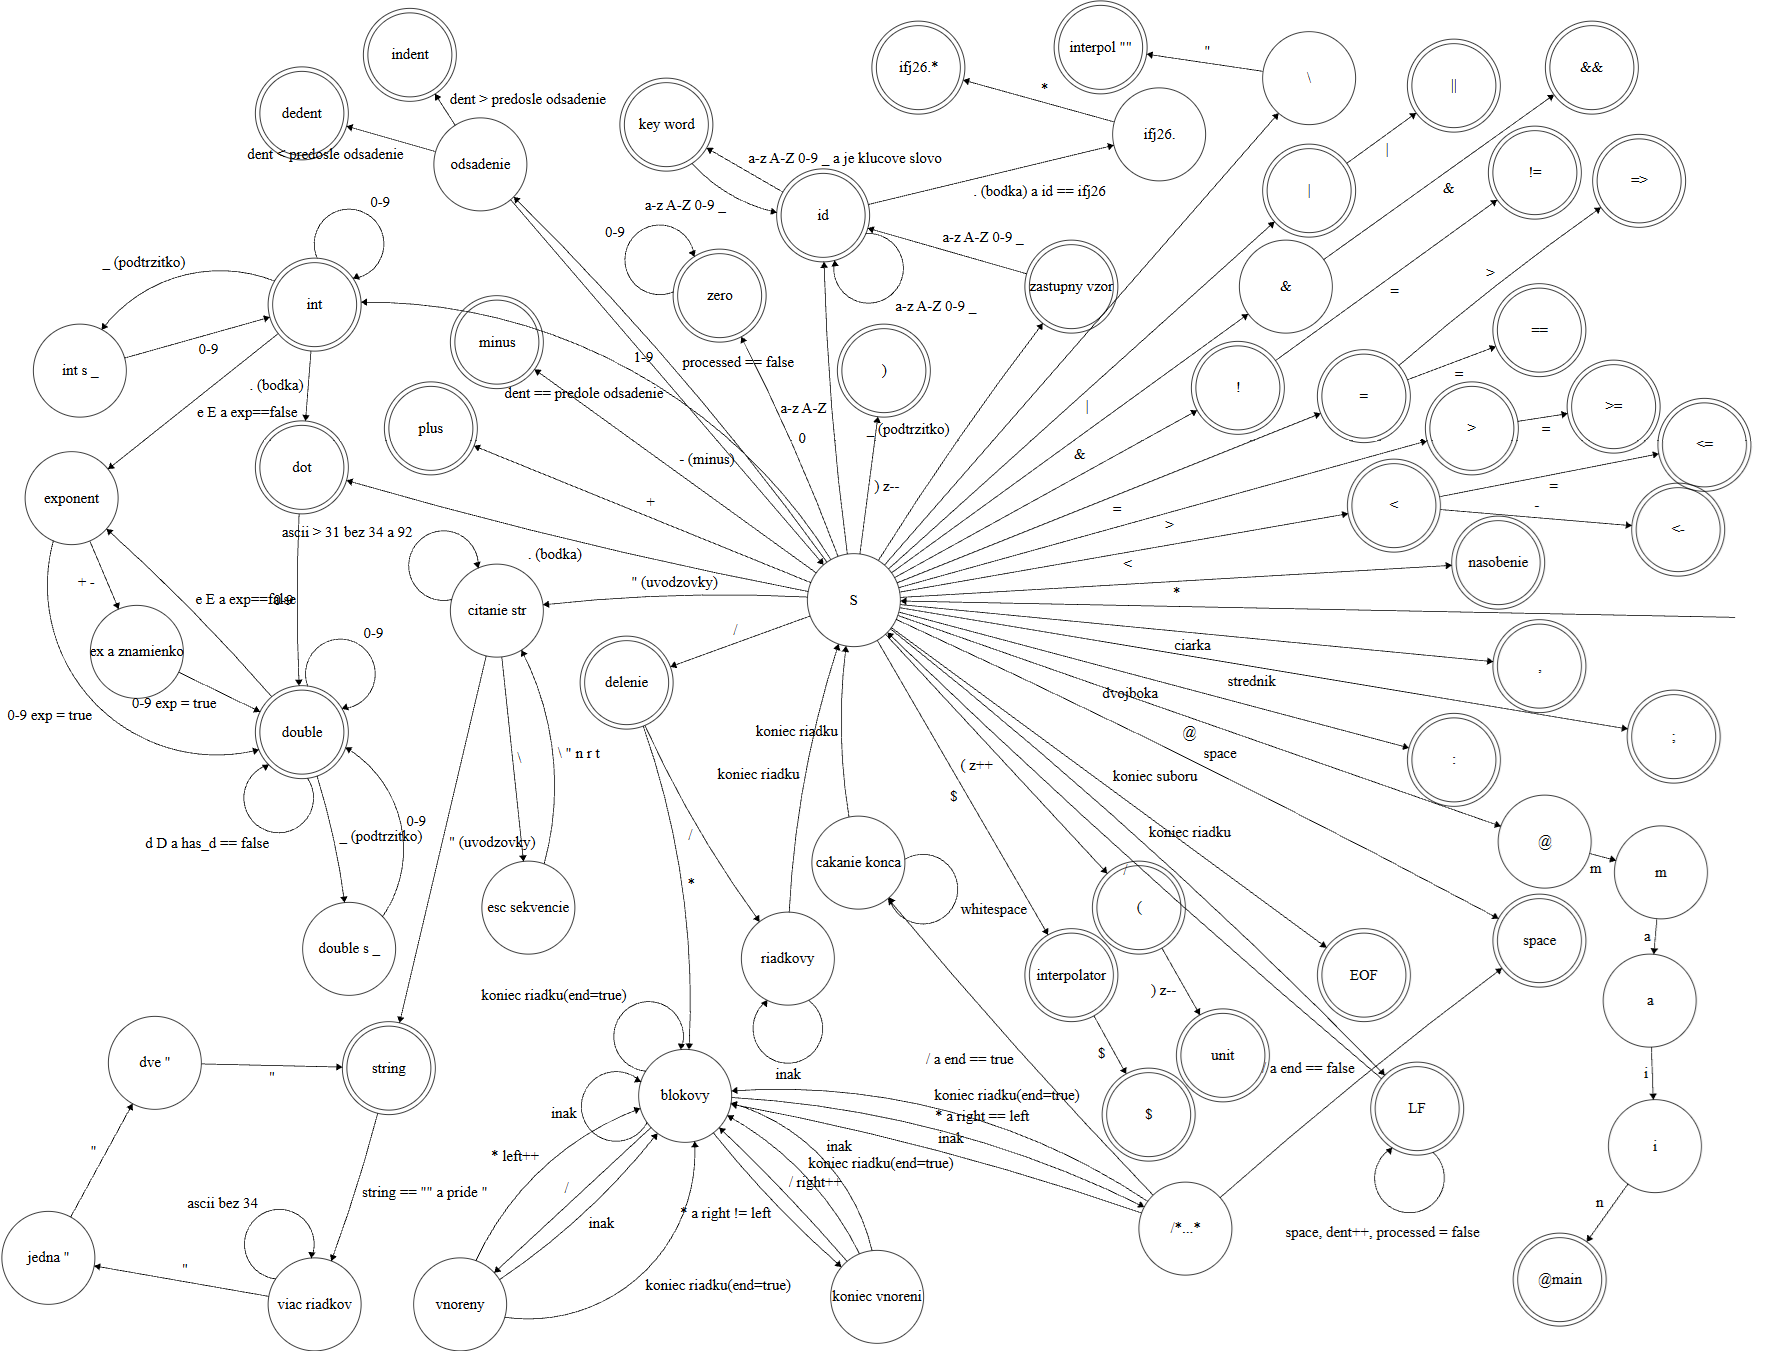
\includegraphics[width=\linewidth,height=0.9\textwidth,keepaspectratio]{KA.png}
  \caption{Konečný stavový automat lexikálnej analýzy.}
  \label{fig:ka}
\end{sidewaysfigure}

\section{Popis modulov}

\begin{description}
    \item[\texttt{scanner.c/.h}] Lexikálny analyzátor implementovaný ako deterministický konečný automat, ktorý odsadenie prevádza na tokeny \texttt{INDENT}/\texttt{DEDENT} pomocou zásobníka úrovní odsadenia.

    \item[\texttt{syntactic.c/.h}] Syntaktický analyzátor implementovaný metódou rekurzívneho zostupu podľa LL gramatiky, s jedným tokenom dopredu. Pri čítaní stavia derivačný strom. Vnútri zátvoriek považuje konce riadkov a zmeny odsadenia za biele znaky. 
    Poznámka \footnote{LL Gramatika pôvodne obsahovala všetky rozšírenia (okrem LISTS), avšak neskôr sme sa rozhodli určité rozšírenia neimplementovať. To malo za následok, že v syntaktickom analyzátore sú implementované všetky rozšírenia (- LISTS).}.
    
    \item[\texttt{precedence.c/.h}] Precedenčná syntaktická analýza výrazov zdola nahor. Rieši volania funkcií a prístup k členom cez bodku. Volá ju rekurzívny zostup na miestach, kde čaká výraz.

    \item[\texttt{tree.c/.h}] Všeobecný n-árny derivačný strom. Vnútorné uzly nesú číslo použitého pravidla gramatiky a listy kópiu tokenu. Slúži ako spoločná dátová štruktúra medzi syntaktickou analýzou, sémantickou analýzou a generátorom.
    
    \item[\texttt{symtable.c/.h}] Tabuľka symbolov používa hašovaciu funkciu djb2, začína na veľkosti 97 a po prekročení zaplnenia 60\,\% sa zdvojnásobí. Pre premenné ukladá typ a meniteľnosť (\texttt{var}/\texttt{val}), pre funkcie typy parametrov a návratový typ.

    \item[\texttt{semantics.c/.h}] Sémantická analýza prebieha v niekoľkých prechodoch nad stromom: najprv zber tried, typových aliasov a funkcií, potom kontrola funkcie \texttt{main} a nakoniec typová kontrola výrazov, premenných... Výsledky ukladá do pomocnej štruktúry pre generátor. Každý rozsah má vlastnú tabuľku premenných. 

    \item[\texttt{generator.c/.h}] Generátor výrazy vyhodnocuje zdola nahor na dátovom zásobníku. Každá deklarácia dostane poradové číslo, vďaka čomu sa premenné s rovnakým názvom ale z iných častí kódu neprekrývajú. Argumenty funkcií a návratová hodnota sa odovzdávajú cez dátový zásobník.

    \item[\texttt{main.c}] Vstupný bod prekladača, ktorý postupne spustí syntaktickú analýzu (spolu s lexikálnou), sémantickú analýzu a generovanie kódu na štandardný výstup. 
\end{description}

\section{Použitie AI}
Pri práci na projekte sme využívali jazykový model Claude Opus~5.5 (Claude Code/claude.ai), a~to najmä na:
\begin{itemize}
  \item \textbf{debugging} -- ak niektorá časť prekladača nefungovala podľa očakávania, s~pomocou AI sme hľadali, prečo je kód chybný a~ako ho opraviť.
  \item \textbf{prepis gramatiky do kódu} -- prepis časti gramatických pravidiel na funkcie syntaktického analyzátora podľa predlohy.
  \item \textbf{generovanie \LaTeX{} kódu dokumentácie} -- napr. sadzba tabuliek a~ich formátovanie, samotný text ani obsah tabuliek AI negenerovala.
  \item \textbf{testovanie} -- generácia a testovanie testovacích skriptov a zdrojových kódov v IFJ26.
\end{itemize}

\begin{thebibliography}{9}
  \bibitem{djb2}
    YIGIT, Ozan. \textit{Hash Functions} [online]. Toronto: York University. 
    Dostupné z:~\url{http://www.cse.yorku.ca/~oz/hash.html}.
\end{thebibliography}

\end{document}
